%
\subsection{FOCMEC}
\label{sect:focmec}

The program can be used to determine double couple earthquake focal 
mechanisms using polarities and/or amplitude ratios for both local 
and global earthquakes. The program also provides an interactive 
graphical display. The existing solution can be plotted without any 
station data or location being available, however if existing polarities 
should be plotted, the event must be locatable in order to calculate 
angles of incidence. Several solutions can be plotted on the same 
figure in order to compare solutions.

The SEISAN program FOCMEC provides the interface between the database 
and the program that determines focal mechanisms, which in SEISAN is 
the program FOCMEC\_EXE. This program is written by Arthur Snoke 
\citep{snoke1984} 
and distributed as part of the FOCMEC package 
(\url{http://www.geol.vt.edu/outreach/vtso/focmec}). 
FOCMEC\_EXE is identical to FOCMEC in Snoke's package and can be 
easily upgraded (unless formats are changed). Generally the user 
will use FOCMEC when working with SEISAN data, however, it is also 
possible to run the original version (see documentation by Snoke: 
INF/focmec.pdf).
%\textcolor{red}{lo-change: 
Before FOCMEC\_EXE is started the
user can optionally change the inputfile \texttt{focmec.run}.

\index{Polarity}

The program works with polarities and amplitude ratios. See the MULPLT section 
on how to read polarities and amplitudes.  Note that since amplitude 
ratios are used, there is no need to correct for instrument response 
provided the response is the same for the different components (within 5-10 \%).

Use of amplitudes

Amplitude ratios are computed from amplitude readings given in the S-file. While amplitude ratios can provide additional constraint on the solution, they should be used with caution. Ideally, the solution should be well constrained by polarities only, and then amplitude ratios can provide confirmation of a solution or help to select one of several equally good solutions. The principle behind the amplitude ratio method is that the effect of geometrical spreading will cancel out when forming the amplitude ratios of S and P waves (or SV/SH) of the same phase type, e.g. Pg and Sg. This leaves the following corrections  to be made  on the amplitudes before the ratios are calculated.

\begin{itemize}
\item
Calculate angle of incidence at the station and correct for the free surface effect.
\item
For local earthquakes, use the calculated travel time for a particular phase to correct for Q. Different Q for P and S can be used and the frequency used is the frequency of the maximum amplitude phase.
\item
For distant earthquakes, correct for $t^{*}$. Different $t^{*}$ for P and S can be used.  The frequency used is the frequency of the maximum amplitude phase.
\end{itemize}

The attenuation parameters have default values of:

\begin{displaymath}
\begin{array}{ll}
Q = 100 \times f^{1.0} & \textrm{for P and S-waves}\\
t^{*} = 1.0 & \textrm{for P-waves}\\
t^{*} = 4.0 & \textrm{for S-waves}
\end{array}
\end{displaymath}

Different values can be set in file FOCMEC.DEF, which can be located in DAT or working directory.

The observations to be made are:

\begin{itemize}
\item
Rotate the seismogram (if three component record) to get R and T components.
\item
Read maximum amplitude P-phase and corresponding period on Z, phase P.
\item
Read the  maximum amplitude S-phase (same type) and corresponding period on Z, phase (SV).
\item
Read the  maximum amplitude S-phase (same type) and corresponding period on H, phase (SH).
\end{itemize}

The wave type Pg/Sg or Pn/Sn has to be given when the amplitude is read. When reading on uncorrected seismograms, MULPLT will want a confirmation that the user wants to save uncorrected amplitudes, since, normally, all amplitude observations in an S-file are in nm. It is possible to filter the signals provided the same filter is used for P and S. Ideally, the amplitude observation should be made at a frequency below the earthquake corner frequency and consequently also the filter high cut frequency should  be below the corner frequency.

It is also possible to read amplitudes on the radial component. However, SV amplitudes and phases change rapidly around the critical angle and the amplitudes can therefore be unreliable (see INF/focmec.pdf for details). So, although SEISAN will use the amplitudes read on the radial component, it is in general not recommended to use them. Assuming reading on only Z and H, the following amplitude ratios are calculated:

\begin{itemize}
\item
SV/P
\item
SH/P
\item
SV/SH
\end{itemize}

In reality, the data only provides 2 independent ratios so ideally only 2 should be used. Since it is hard to know which 2 are the most reliable, SEISAN uses all. 

Phase names in SEISAN used for amplitudes for FOCMEC have the names AMPG, AMSG, AMPN and AMSN for direct and first arrival (refracted), respectively. For local earthquakes both PG and PN types can be used while for distant earthquakes only PN types can be used.

Polarity selection

Any P-phase (first letter of phase name is P) with a polarity (C or D) is used, like P, Pg, PP etc. For further processing in FOCMEC, C  is labeled C if phase onset is ' ' or I and '+' if phase onset is E. Correspondingly, polarity D is labeled D or -.   FOCMEC can also use polarities of SV and SH, but this has not been implemented in SEISAN.

Local earthquakes

Any P-phase can be used like Pn and Pg. When few polarities are available, it is an advantage to use both Pg and Pn since these phases have different angles of incidence. Polarities associated with other phases are not used. There is no check if a P-phase has been duplicated. \newline
Amplitude ratios must be determined from the same wave type for example Pg and Sg and the program will only form amplitude ratios from the same wave types.  While in principle it should be possible to use ratios determined from refracted waves, generally ratios determined only from direct waves are used since they are easier to identify and have larger amplitudes than refracted arrivals. Particularly the Sn is difficult to identify. This means that the amplitudes readings most often will be made within what is considered the maximum amplitude in the Pg and Sg wave trains. However, the polarity might be read on the first arrival which can be Pn or another refracted arrival. 

Distant earthquakes

Polarities of any P-phase can be used (but not pP since first letter is not P ). Using amplitudes require events with clear P and S phases and usually this means reading on broad band records. The amplitude phase names AMPN/SN are used to indicate first arrivals.


Program operation

The program makes a grid-search and finds how many polarities and amplitude ratios fit each possible solution. All solutions with less than a given number of wrong polarities and/or amplitude ratios within given error limits, are then written out and can be plotted. With a cursor, the user can then select the preferred solution, which can be stored in the input file or the database.  The program is intended to work from within EEV (option F), however it can also work independently (see below). The program uses an input file called \texttt{focmec.inp} (automatically generated). This is a Nordic format file. Direct waves have angle $>90$ and refracted arrivals angle $<90$ degrees. If the angle is $>90$, the polarity is plotted at an azimuth+180. If the user wants to use FOCMEC as a freestanding program, the angle of incidence information may have to be put in manually in a standard CAT-file, which is then renamed focmec.inp. This can be done automatically by FOCMEC if a \texttt{hyp.out} and corresponding print.out file is available. 
FOCMEC can also be used to convert angles, like dip, strike and rake to T and P-axis, simply say 'focmec a', where argument a stands for angles and you will be prompted for input.

%The program makes a grid-search and finds how many polarities fit each possible solution. All solutions with less than a given number of wrong polarities and/or amplitude ratios within given error limits, are then written out and can be plotted. With a cursor, the user can then select the preferred solution, which can be stored in the input file or the database.  The program is intended to work from within EEV (option F), however it can also work independently (see below). The program uses an input file called focmec.inp. This is a Nordic format file. The angle of incidence is put in column 58:60, format I3 (although from version 8 onwards, this information is part of the S-file). Direct waves have angle > 90 and refracted arrivals angle <90 degrees. If the angle is >90, the polarity is plotted at an azimuth+180. If the program is operated from within EEV, this information is automatically put in and the \index{Focmec.inp}focmec.inp file created. If the user wants to use FOCMEC as a freestanding program, the \index{Angle of incidence }angle of incidence information must be put in manually in a standard CAT-file, which is then renamed focmec.inp. This can be done automatically by FOCMEC if a \texttt{hyp.out} and corresponding \texttt{print.out} file is available.  FOCMEC can also be used to \index{Convert angles}convert angles, like dip, strike and rake to \index{T and P-axis}T and P-axis, simply say `focmec a', where argument a stands for angles and you will be prompted for input. 

\index{Focmec.inp}
\index{Angle of incidence}
\index{Convert angles}
\index{T and P-axis}

When the program runs, all amplitude information and corresponding corrections are listed:

\begin{verbatim}
============ FOCMEC ============
No FOCMEC.DEF file, use defaults

Q: Local: Qp= 100.0**1.00  Qs= 100.0** 1.0   Global: t*(P)=1.00  t*(S)=4.00

STAT  C PH       AMP    PER TRTIME   QCOR ANGINC ANGEMG Fcor   AZ  DIST
SNART Z PG      1582   0.16   12.6    1.2    100     79  0.6  301    77
SNART Z SG      9397   0.19   21.8    1.3    100     79 -0.3  301    77
SNART T SG     10577   0.09   21.8    1.3    100     79  2.0  301    77
MUD   Z PG        53   0.10   26.3    1.4     94     85  0.3  163   179
MUD   Z SG       197   0.15   45.5    1.7     94     85 -0.2  163   179
MUD   T SG       209   0.22   45.5    1.6     94     85  2.0  163   179
BLS5  Z PG       749   0.28   28.0    1.3     94     85  0.3  326   192
BLS5  T SG      1102   0.10   49.8    1.9     94     85  2.0  326   192
BLS5  Z SG       662   0.10   49.8    1.9     94     85 -0.2  326   192

 STAT  Ratio type  T     Amp 1    Amp 2  Fcor LogRat
 SNART SV(Z)/P(Z)  V      9397     1582   1.0   0.80
 SNART SH(T)/P(Z)  H     10577     1582   0.3   0.34
 SNART SV(Z)/SH(T) S      9397    10577   3.5   0.47
 MUD   SV(Z)/P(Z)  V       197       53   1.3   0.75
 MUD   SH(T)/P(Z)  H       209       53   0.2  -0.12
 MUD   SV(Z)/SH(T) S       197      209   7.5   0.87
 BLS5  SH(T)/P(Z)  H      1102      749   0.2  -0.45
 BLS5  SV(Z)/P(Z)  V       662      749   1.3   0.23
\end{verbatim}

%STAT  C PH       AMP    PER TRTIME   QCOR ANGINC ANGEMG   AZ  DIST
%SNART R PG       202   0.22   15.4    1.6     99     80    2    94
%SNART T SG       949   0.10   26.2    2.3     99     80    2    94
%SNART Z SG       656   0.15   26.2    2.3     99     80    2    94
%SNART R SG      1039   0.09   26.2    2.3     99     80    2    94
%MUD   Z PG        32   0.18   25.1    2.2     95     84  132   170
%MUD   T SG       231   0.10   43.5    3.9     95     84  132   170
%MUD   Z SG       164   0.08   43.5    3.9     95     84  132   170

%STAT  Ratio type  T     Amp 1    Amp 2  Fcor LogRat
%SNART SH(T)/P(R)  H       949      202   0.7   0.65
%SNART SV(Z)/P(R)  V       656      202   2.8   1.10
%SNART SV(R)/P(R)  V      1039      202   4.6   1.52
%SNART SV(Z)/SH(T) S       656      949   4.2   0.46
%SNART SV(R)/SH(T) S      1039      949   6.9   0.88
%MUD   SH(T)/P(Z)  H       231       32   0.2   0.35
%MUD   SV(Z)/P(Z)  V       164       32   1.2   1.05
%MUD   SV(Z)/SH(T) S       164      231   7.1   0.70

The abbreviations are STAT: Station code, C: Component, PH: Phase, AMP: Amplitude in count, PER: Period in sec, TRTIME: Travel time in sec, QCOR: Log Q-correction, ANGINC: Angle of incidence at the source, ANGEMG: Angle of emergence at the station, 
%\textcolor{red}{jh-change:
Fcorr: Free surface correction for this amplitude, 
Az: Azimuth from the event to the station, DIST: Epicentral distance in km., Ratio type (see text), T: indicator of ratio type, Amp1 and Amp2: The two amplitudes (count) in the ratio, Fcor is the free surface correction in the amplitude ratio (to be multiplied with ratio) and LogRat is the logarithm of the corrected amplitude ratio used.

Note that for station SNART, amplitudes were also read on the radial component so more then 3 amplitude ratios were used.

Following, the user get the choices:

%When the program runs, the following menu is put up: 

\begin{verbatim}
Stop                        (0)
Plot saved solution(s)      (1)
Plot new solutions          (2)
Plot selected solution      (3)
Find new solutions          (4)
-1, -2, -3 also plot station 
\end{verbatim}

\begin{enumerate}
\item
This is the solution(s) already stored in the data base (S-file). 
%The idea is that there should only be one prime fault plane solution. The prime solution has ' F' in the last two columns of the line. If any other character is put into column 79, the solution is not considered prime, however it will be left in the file when new solutions are generated.  There might be a need to plot several solutions in order to compare solutions. In that case the character in column 79 must be 'O'.
% \textcolor{red}{jh-change:
See secetion "Storing and selecting fault plane solutions" below.
%This is the solution(s) already stored in the data base (S-file). The rule is that there should only be one prime fault plane solution. The prime solution has ` F' in the last two columns of the line. If any other character is put into column 79, the solution is not considered prime, however it will be left in the file when new solutions are generated. There might be a need to plot several solutions in order to compare solutions. In that case the character in column 79 must be `O'.
\index{Fault plane solution, plotting several} 
\item
Plotting new solution after having used option 4 
\item
Plotting the selected solution after using option 4 \newline
Using e.g. -1 instead of 1, also plots the stations to 
help identify them on the plot, see Figure \ref{fig:focmec} 
\item
Starting a search for new solutions 

Option 4 gives the following information and questions: 

\begin{verbatim}
There are   10 polarity readings
Maximum number of allowed polarity errors or -1 to show best solutions only
\end{verbatim}

Depending on number of data values, 0-5 is a good answer. To let the program find the minimum number of polarity errors, type '-1', which is particular useful if there is a significant minimum number of polarity errors.

\begin{verbatim}
There are  8 amp ratio readings
Maximum number of allowed amplitude ratio errors
\end{verbatim}

Equivalent for ratios to 'Maximum number of polarity errors', however, error is defined by amplitude ratio error. Number of errors depends on number of observations. For 9 observations 1-2 errors is reasonable.

\begin{verbatim}
Maximum amplitude ratio error,  return for default of .2
\end{verbatim}

Give maximum allowed difference between observed and computed log amplitude ratio, default is 0.2, which often is a good value.

\begin{verbatim}
Degree increment in search
\end{verbatim}

%Number of polarity values: Number of polarities found for event with P-phases.  \newline
%Any P-phase can be used like Pn and Pg. When few polarities are available, it is an advantage to use both Pg and Pn since these phases have different angles of incidence. Polarities associated with other phases are not used. There is no check if a P-phase has been duplicated.  

%Number of amplitude ratios: Total number of amplitude ratios derived from amplitude readings in S-file. 

\end{enumerate}

%The program now asks:
%
%Maximum number of polarity errors: Depending on number of data values, 
%0-5 is a good answer. To let the program find the minimum number of 
%polarity errors, type `-1', which is particular useful if there is 
%a significant minimum number of polarity errors. \newline
%Maximum number of amplitude ratio errors: Equivalent for ratios to 
%`Max number of polarity errors', however, error is defined by 
%amplitude ratio error. \newline
%Maximum amplitude ratio error: Give maximum allowed difference between observed and computed amplitude ratio, default is 0.2. 
%
%Degree increment in search: Initially use e.g. 20 deg to make a fast 
%search, later use e.g. 5 deg to make a final solution. \newline

The program will now start the searching and write out on the screen (and in a file) the solutions which fit the requirement of number of misfits. The maximum number of solutions is limited to 100 as a default, or to the value defined by `FOCMEC MAXSOL' in \texttt{SEISAN.DEF}. At the end, the number of acceptable solutions is written out as well as the minimum number of bad fits. This can then be used for the next search. Now option 0 to 4 can be used again. 

When plotting the solution with option 2, the cursor comes up. Also, the solutions will be printed in text 
form to the screen, 
%\textcolor{red}{jh-change: 
see Figure 
\ref{fig:focmec}.
%, e.g.: 

%.\begin{verbatim}
%%.   Strike       Dip     Rake Pol: P      SV    SH   Rat Err  RMS RErr   RErr (All)
%. 358.0200   15.7900  -71.3200     1   0.0   0.0        0      0.25      0.25 
%. 358.1700   28.9000  -57.6200     1   0.0   0.0        0      0.09      0.09 
%.\end{verbatim}

The abbreviations are Pol: Number of polarity errors for P, SV(not used) and SH(not used), Rat Err: Number of ratio errors, RMS RErr: The RMS error for the ratios used, RErr (All): The RMS error for all ratios.

The polarities and amplitude ratios can be plotted on the focal sphere 
using the same convention as the original FOCMEC program, which is: 

\begin{tabular}{ll}
o = & compression \\
+ = & emergent compression \\
$\Delta$ = & dilatation \\
- = & emergent dilatation \\
V = & amplitude ratio SV/P \\
S = & amplitude ratio SV/SH \\
H = & amplitude ratio SH/P \\
\end{tabular}

%The last three fields Rat Err, RMS Rerr and Rerr refer to the number of ratio errors, the RMS error for the ratios used and the RMS error for all ratios, respectively. 

%When saving a solution, the same text field is included into the S-file. 

The user can select a preferred solution by moving the cursor near one of the letters T or P (T and P axis). By pressing T, the program will find the nearest T axis (same for P and nearest P-axis) and corresponding fault plane solution, which can be stored in the database and/or plotted with option 3. If no solution is to be selected, press q for quit. If a solution has been selected, the user will be asked if it is to be saved or not after selecting option 0. The saved solution goes into the 
\index{Focmec.out}
focmec.out and from there into the S-file (type F-line) in the database if FOCMEC is operated from EEV
%\textcolor{red}{jh-change: 
and the solutiosn will also be written to fps.out. 
%NOTE: The previous fault plane solution will be overwritten unless a character is written in column 79 of the fault plane solution line. If e.g. the last 2 characters are `OF', this solution remains in the S-file. 

When working from EEV, the event will always be located before the FOCMEC program starts up. In 
the Nordic format the solution is stored simply as 
\index{Strike}
strike, 
\index{Dip}
dip, 
\index{Rake}
rake and number of bad polarities (3f10.1,I5). Aki and Richards convention is used. In addition, the name FOCMEC will be written near the end of the line to indicate that the fault plane solution was made by FOCMEC. The other program, which can make a fault plane solution, is INVRAD (see EEV). The line type is F. 

The following files are created: 

\texttt{focmec.dat}: Input parameters to FOCMEC\_EXE. \newline
\texttt{focmec.log}: Log of the FOCMEC\_EXE run. \index{focmec.lst}\newline
\texttt{focmec.lst}: More details on solutions \newline
\texttt{focmec.out}: Gives input parameters and solutions \index{Focmec.eps}\newline
\texttt{focmec.eps}: A Postscript plot file of LATEST plot  \newline
\texttt{focmec.run}: Run parameters for FOCMEC\_EXE, you can re-run FOCMEC by `focmec\_exe < focmec.run' 

\textbf{Running FOCMEC independently of EEV and composite fault plane solution:}
\index{Fault plane solution, composite }

Locate event(s) with HYP, then give command focmec. The program then combines the files \texttt{print.out} and \texttt{hyp.out} \index{Hyp.out}to make the focmec.inp file and proceeds as usual. This is actually the way FOCMEC works from within EEV. However, if more than one event is located, FOCMEC assumes that all events shall be used in a composite solution, and focmec.inp will therefore contain the header from the first event and phase lines from all subsequent events. This is the easiest way to make a composite solution. 

NOTE, when running FOCMEC outside EEV, the fault plane solution is not put into the database (it does not belong to any particular event !), however it is written out in file focmec.inp 
%\textcolor{red}{jh-change:
and fps.out. 

Computer limitations: Total number of polarities must be less than the dimension of array DATA (parameter max\_data) for Nordic data (see file \texttt{seidim.inc} in INC directory). 

Figure \ref{fig:focmec} shows an example of a fault plane solution calculated with FOCMEC. 

\begin{figure}
\htmlimage{scale=2.0}
\centerline{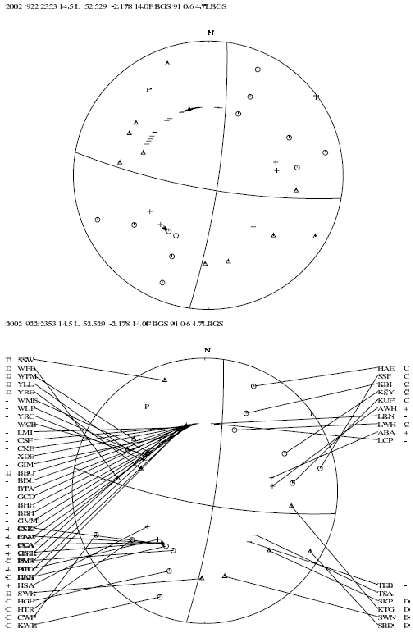
\includegraphics[width=0.9\linewidth]{fig/fig38}}
\caption{Top: An example of a fault plane solution plot. Symbols are explained 
in the text. Bottom: A fault plane solution also showing the stations with corresponding polarities. 
}
\label{fig:focmec}
\end{figure}

